\documentclass{article}
\usepackage[utf8]{inputenc}
\usepackage[T1]{fontenc}
\usepackage{amsmath}
\usepackage{graphicx}
\usepackage{amssymb}
\usepackage{float}
\usepackage{tikz}
\usepackage{pgfplots}
\usepackage[letterpaper, margin=1in]{geometry}

\title{Concealed Bike Anti-Theft Device: Design Document}
\author{Elizabeth Atkinson (eatkinso)\\ Srinidhi Raman (nidhim2) \\ Alex Wen (acwen2) }

\begin{document}

\section{Introduction}
\subsection{Problem}

\paragraph{}
College students frequently face the issue of bikes being stolen on campus. Even with the strongest of protections, they are not completely capable of deterring thieves who have various equipment. Our own member, Elizabeth, had her bike secured with a substantial solid steel U-lock, but was stolen regardless last fall, when someone apparently sawed through the u-lock at night. 

In order to discourage bike theft, it would be useful to have a bike anti-theft device that could enable the user to track the bike's location wirelessly

\subsection{Solution Overview}
\paragraph{}
We propose a concealed bike anti-theft device that helps bikers prevent their bike from being stolen by unlocking to a specific RFID key (therefore difficult to mimic), providing GPS tracking so the user has the ability to track down the bike if stolen, and frightening away potential thieves with a loud noise when theft is detected.

The device will receive GPS coordinates and periodically transmit the coordinates over LoRa to be received by the user. To allow the bike system to differentiate between potential thieves and the owner, the owner of the bike will have an RFID tag such that while the user is on the bike, the RFID tag can be detected. If the bicycle is moved when the RFID tag is not nearby, it will trigger a loud and annoying alarm to scare away the potential thief.

The device will be designed in a manner such that it is difficult to find and remove, discouraging potential bike thieves from removing the bike. Additionally, the device will be designed to fit a relatively universal bike structure, which will allow the device to be attached to any bike. A standardized device will be more convenient for users as bikes with integrated tracking systems tend to be very expensive.

Our device will be small, rechargeable, battery-powered, and enclosed in a weatherproof enclosure that can easily be attached to most bikes.
\subsection{High-Level Requirements}

\begin{enumerate}
	\item If a user tries to remove the bike from a stationary location without the RFID tag, the alarm will sound. 
	
	\item The device receives GPS data \textit{at least} once per minute, and records its own position over time.  
	
	\item The device transmits its GPS location data and additional data over LoRa to be received by a base station. 
	
\end{enumerate}

\section{Design}
\subsection{Overall System Block Diagram}
\begin{figure}[H]
	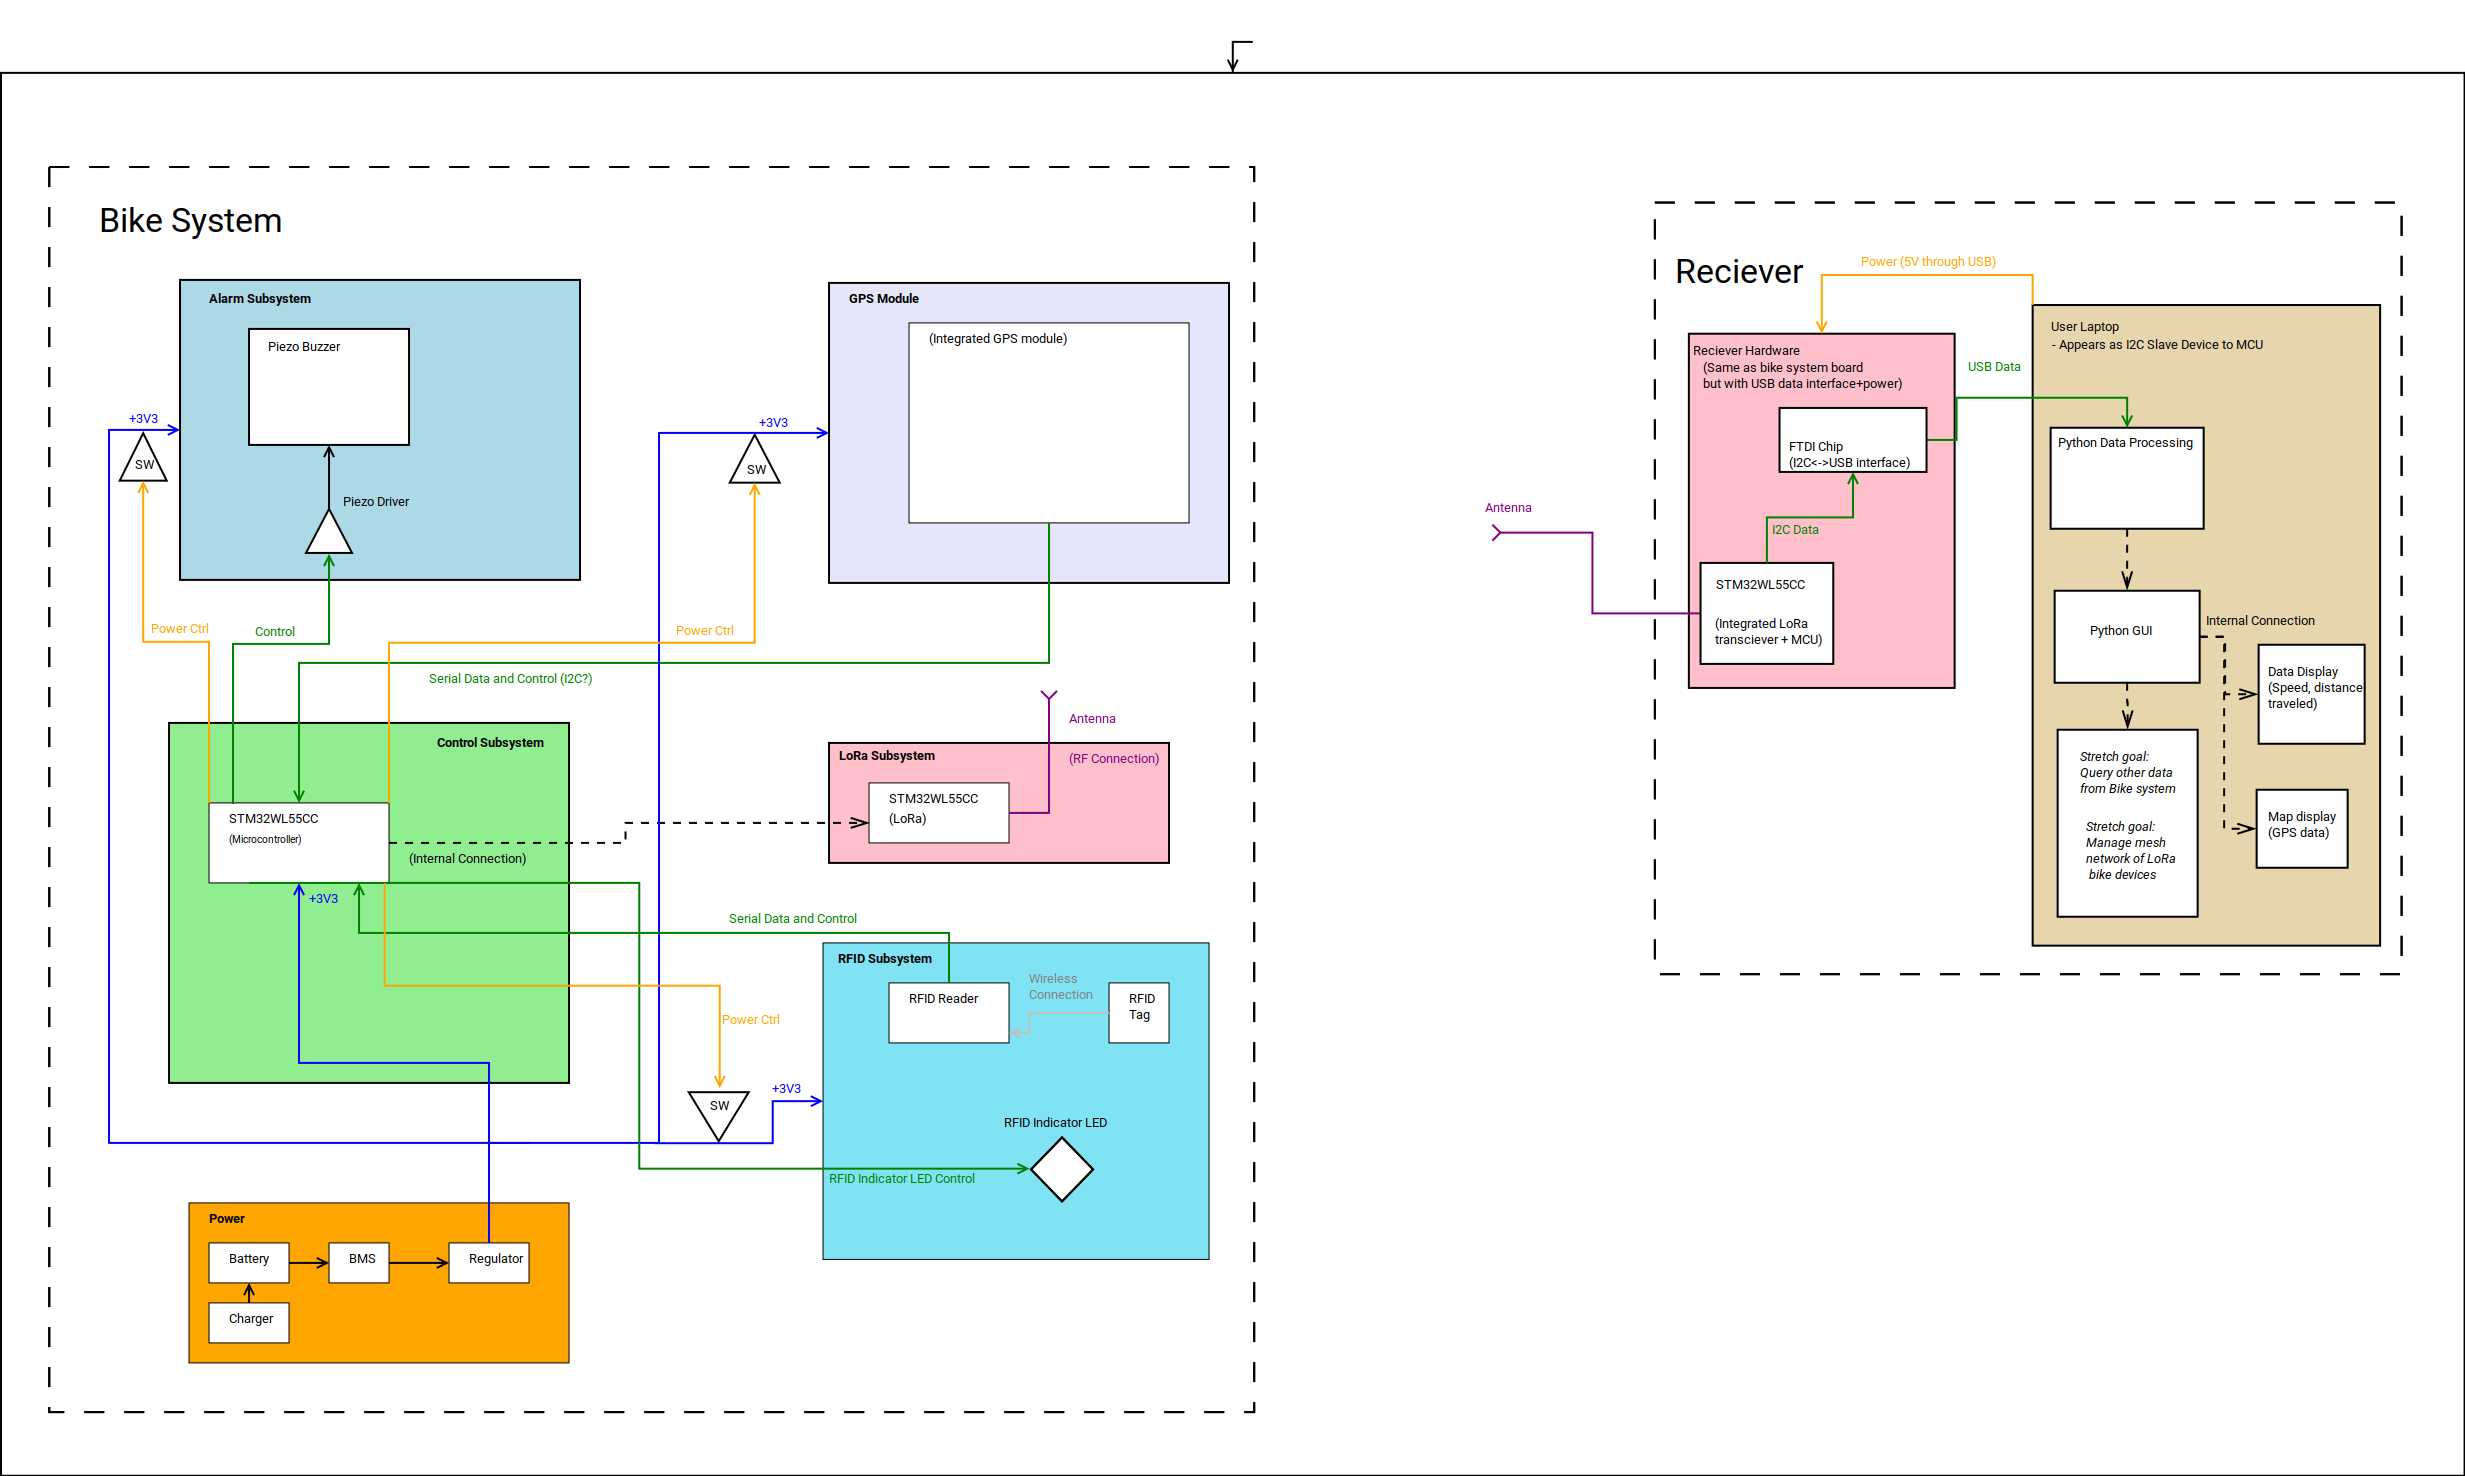
\includegraphics[width=\textwidth]{block_diagram_full.png}
	\caption{Full Block Diagram}
\end{figure}


\subsection{Physical Design}

\subsection{Subsystem Designs} 
\subsubsection{On-Bike Control System}

\paragraph{}
We will use the STM32WL55CC, an SoC that includes both a dual-core ARM microcontroller and a wireless transceiver \cite{stm_datasheet}. The microcontroller will be responsible for buffering data from the GPS receiver, packetizing the data to send over LoRa, and internally transferring the data to the integrated RF transceiver. The microcontroller will also manage the control signals for the alarm subsystem, RFID subsystem, and GPS module. 

Since this is a battery-powered device, the microcontroller will also be responsible for implementing power-saving measures. For example, the microcontroller will vary the number of GPS data transmissions depending on the bike state: while the bike is in a “idle/safe” state (stationary in one location) it will only transmit its location over LoRa once per hour. If the device is in the “stolen” state, it will transmit its location over LoRa once per minute. The microcontroller will also cut off power to the Alarm when it is not in use, and as a stretch goal, the microcontroller will selectively cut power to the RFID/GPS subsystems in an intelligent manner (ie, the RFID transmitter will not continuously transmit/listen for the RFID tag if the GPS module detects that the bike is in motion, and the motion was initiated by the correct user). 
\paragraph{} 

\textit{\textbf{Control Subsystem Requirements:}}

\begin{enumerate}
	\item The microcontroller implements a state-based control system with power-saving measures in the idle/safe states. 
	\item The microcontroller packetizes data to be sent over LoRa at an update rate of \textit{at least }once per hour in “idle” states, and \textit{at least} once every two minutes in “active” states. 
	\item \textit{Stretch goal:} The microcontroller manages multi-unit mesh networking by re-transmitting received data within 1 second of receiving the data. (See the \textbf{LoRa Subsystem} section for more detail on mesh networking). 
\end{enumerate}



\begin{thebibliography}{}
	\bibitem{ethics} IEEE, "IEEE Code of Ethics," \textit{IEEE}, 2022. Available: https://www.ieee.org/about/corporate/governance/p7-8.html. [Accessed: Feb. 10 2022].
	\bibitem{LoRA} LoRa Alliance, "What is LoRaWAN: A Technical Overview of LoRa and LoRaWAN", 2015.
	
	\bibitem{gps} GlobalSat. "GlobalSat GPS Module Hardware Data Sheet." Product No: EM-506. 2013. https://cdn.sparkfun.com/datasheets/GPS/EM506\_um.pdf
	
	\bibitem{rfid} ID-innovations. "ID-3LA, ID-12LA, ID-20LA Low Voltage Series Reader Modules." 2015. https://cdn.sparkfun.com/assets/c/7/0/e/3/DS-11828-RFID\_Reader\_ID-20LA\_\_125\_kHz\_.pdf
	
	\bibitem{reflector} Photograph by Julo, public domain, Wikimedia Commons Available: https://upload.wikimedia.org/wikipedia/commons/b/b1/BicycleRetroreflectors.JPG. [Accessed: Feb 10 2022]. 
	\bibitem{matchingAN} STMicroelectronics, "RF matching network design guide for STM32WL Series", AN5457, 2020. 
	\bibitem{stm_datasheet} STMicroelectronics, "Multiprotocol LPWAN dual core 32-bit Arm® Cortex®-M4/M0+	LoRa®, (G)FSK, (G)MSK, BPSK, up to 256KB Flash, 64KB SRAM", DS13293, 2021.
	
	
	
	\bibitem{battery} Wikipedia, "List of Battery Sizes", 2022. [Online]. Available: https://en.wikipedia.org/wiki/List\_of\_battery\_sizes. [Accessed: 10 Feb 2022]. 
	
	
	
\end{thebibliography}
\end{document}
